\section{Systematic Uncertainties}
\label{sec:llvv_systematics}

This section summarizes the experimental and theoretical sources of systematic uncertainty affecting the event yields of both the signal and background processes, and their impact on the total and differential cross-section measurements.

The systematic uncertainties are evaluated to account for residual discrepancies between data and simulation in the modelling of trigger efficiencies, lepton reconstruction and identification, jet calibration, $b$-tagging, missing transverse energy ($E_{\text{T}}^{\text{miss}}$), the integrated luminosity, and the average number of proton--proton interactions per bunch crossing (pile-up). In addition, theoretical uncertainties are considered, including those arising from the choice of parton distribution functions, renormalization and factorization scales, higher-order corrections, and the modelling of parton shower and hadronization.

Consistent with previous analyses of the $\text{ZZ}jj$ final state, the measurement of the signal yields and the resulting cross-sections is dominated by statistical uncertainty. Among the systematic sources, the largest contributions arise from jet reconstruction, particularly pile-up suppression and $\eta$-intercalibration, as well as from the unfolding procedure.
%The bias associated with the unfolding method is evaluated through the data-driven closure test discussed in Section~\ref{sec:unfolding_ddclosure}.

\subsection{Experimental Sources}
\label{subsec:exp_syst}

The experimental systematic uncertainties encompass detector effects and reconstruction efficiencies. For each source, the propagation to the final measurement is performed as follows:
\begin{enumerate}
    \item A detector-level SM distribution is constructed using MC predictions where the specific systematic parameter has been varied.
    \item The nominal background is subtracted from this varied distribution.
    \item The resulting background-subtracted distribution is unfolded using the \textit{nominal} response matrix.
    \item The systematic uncertainty is defined as the difference between this unfolded distribution and the nominal MC particle-level (truth) distribution.
\end{enumerate}

To ensure that upward and downward variations are statistically significant and symmetric, bootstrap replicas are utilized. In cases where the variations are symmetric within statistical uncertainties, the final systematic value is smoothed by averaging the absolute values of the variations.

The specific sources considered are listed below:

\begin{itemize}
    \item \textbf{Luminosity:} 
    The total integrated luminosity of the dataset is known to a precision of $0.83\%$. This uncertainty is determined using a combination of van der Meer beam separation scans in dedicated data-taking sessions and calibrated luminosity-sensitive detectors during regular data-taking periods~\cite{DAPR-2021-01}.
    
    \item \textbf{Pile-up Reweighting:} 
    The number of proton--proton interactions per bunch crossing is modelled in simulation by reweighting events to match the distribution observed in data. An uncertainty arises from the limited precision in the ratio of predicted to measured inelastic cross-sections within the ATLAS acceptance region~\cite{STDM-2015-05}. To account for this, a systematic uncertainty \texttt{PRW\_DATASF} is evaluated by varying the scale factor used to reweight the average number of interactions in the simulation by its associated uncertainty.

    \item \textbf{Trigger Efficiency:} 
    Uncertainties in the trigger efficiency scale factors are separated by lepton flavor. For electrons, a single total nuisance parameter is used. For muons, the uncertainty is split into statistical and systematic components.

    \item \textbf{Lepton Efficiency (Reconstruction, Identification, and Isolation):} 
    Efficiencies for lepton reconstruction, identification, and isolation are corrected in simulation using scale factors derived from tag-and-probe control samples in data.
    \begin{itemize}
        \item \textbf{Electrons:} Modeled using a simplified de-correlation model containing 25 nuisance parameters for reconstruction, plus parameters for isolation and identification.
        \item \textbf{Muons:} Involves four uncertainty components covering statistical and systematic terms for both general and low-$p_{\text{T}}$ regimes, plus two parameters for isolation.
    \end{itemize}

    \item \textbf{Lepton Momentum and Scale:} 
    Differences between data and simulation in the lepton momentum scale and resolution are evaluated by applying additional scaling and smearing variations.
    \begin{itemize}
        \item \textbf{Electrons:} Two parameters, \texttt{EG\_RESOLUTION\_ALL} and \texttt{EG\_SCALE\_ALL}, account for electron energy resolution and scale uncertainties derived from $\text{Z} \to \ell^+\ell^-$ samples.
        \item \textbf{Muons:} Independent parameters are used for Inner Detector and Muon Spectrometer measurements, along with Sagitta correction uncertainties and momentum scale parameters.
    \end{itemize}

    \item \textbf{Jet Energy Scale (JES) and Resolution (JER):} 
    Given the hadronic nature of the VBS topology (two forward jets), jet systematics are a dominant source of uncertainty.
    \begin{itemize}
        \item \textbf{JES:} Derived using test-beam data, LHC collision data, and simulation. The \texttt{GlobalReduction} configuration is employed, corresponding to 23 distinct nuisance parameters.
        \item \textbf{JER:} Evaluated by applying additional smearing to the jet energy in simulated samples to match the resolution observed in data. The \texttt{FullJER} configuration (13 parameters) is used.
    \end{itemize}
    
    \item \textbf{Jet Vertex Tagger (JVT):} 
    Scale factor variations for the JVT are applied to account for uncertainties in pile-up jet suppression. Consistent with previous measurements, these variations result in a minor impact ($< 1\%$).

    \item \textbf{Flavor Tagging ($b$-Tagging):}
    The uncertainty in the $b$-tagging efficiency, as well as the corresponding uncertainties in the $c$-jet and light-jet rejection scale factors, are taken into account~\cite{FTAG-2018-01}. These are propagated to the measurement through variations of the flavor-tagging scale factors.

    \item \textbf{Missing Transverse Energy ($E_{\text{T}}^{\text{miss}}$):}
    Uncertainties in $E_{\text{T}}^{\text{miss}}$ are evaluated by varying the soft term (signals not associated with high-$p_{\text{T}}$ objects) and by propagating the lepton and jet energy scale and resolution uncertainties to the $E_{\text{T}}^{\text{miss}}$ calculation.
\end{itemize}

\subsection{Theoretical Sources}
\label{subsec:theo_syst}

Theoretical variations typically induce only minor changes in the shapes of observables but can significantly impact predicted yields. These uncertainties are process-specific.

\begin{itemize}
    \item \textbf{QCD Scale Uncertainties:} 
    These are evaluated using on-the-fly weights corresponding to variations of the renormalization ($\mu_R$) and factorization ($\mu_F$) scales. Seven variations are considered: combinations of $\mu_R$ and $\mu_F$ at factors of 0.5, 1, and 2, excluding the extreme cases where one scale is halved and the other doubled. The envelope of these variations defines the uncertainty. Crucially, for the $\text{ZZ}jj$ signal, the QCD-induced and EW-induced components are treated separately with \textbf{uncorrelated} scale uncertainties.
        
    \item \textbf{PDF and $\alpha_S$:} 
    Uncertainties are evaluated following the PDF4LHC prescription~\cite{Butterworth:2015oua}. This includes the RMS of 100 internal replicas of the NNPDF3.0 set. The effect of the strong coupling constant is assessed separately by varying $\alpha_S$ by $\pm 0.001$ and adding the result in quadrature.

    \item \textbf{MC Generator Modelling:} 
    To assess the uncertainty associated with the MC generator choice for the QCD-induced signal component, the nominal \textsc{Sherpa} sample is compared to an alternative sample generated with \textsc{Powheg}. The relative difference in the unfolded cross-section is taken as a systematic uncertainty.
    
    \item \textbf{Parton Shower:}     
    Uncertainties in the parton showering are calculated within \textsc{Sherpa} by varying the shower recoil scheme. Further details are documented in Ref.~\cite{llvv_partonshower}.

    \item \textbf{$\text{Z}$+Jets Background Normalization:}
    In the $\text{ZZ}jj$ phase space, the $\text{Z}+\text{jets}$ background is estimated using MC simulation. A conservative normalization uncertainty of $50\%$ is assigned to this background to account for potential mismodelling in events with high jet multiplicity. This value is motivated by discrepancies observed in inclusive $\text{Z}+\ge 2$ jets control regions.
\end{itemize}

\subsection{Summary of Impact of the Systematic Uncertainties}

The experimental and theoretical uncertainties are incorporated into the analysis as variations of the corresponding nuisance parameters in a simultaneous fit to the data used to extract the cross-sections. The impact of these uncertainties on the measured fiducial cross-sections for the inclusive ($\text{ZZ} \to \ell\ell\nu\nu$) and VBS-enriched ($\text{ZZ}jj \to \ell\ell\nu\nu jj$) phase spaces is summarized in Table~\ref{tab:uncertainties}.

\begin{table}[htbp]
\centering
%\scriptsize
\renewcommand{\arraystretch}{1.5}
\begin{tabular}{lcc}
\toprule
\textbf{Systematic Source} & \textbf{Impact on $\sigma_{\text{ZZ} \to \ell\ell\nu\nu}$} & \textbf{Impact on $\sigma_{\text{ZZ}jj \to \ell\ell\nu\nu jj}$} \\
\midrule
Scale variation                          & 0.99\%  & 3.5\%   \\
PDF and $\alpha_S$          & 0.15\%  & 0.42\%  \\
Alternative signal generator & 0.38\%  & 0.93\%  \\
$\text{Z}$+jets modelling             & --      & 0.43\%  \\
\midrule
Jet energy scale and resolution & 1.7\%   & 8.7\%   \\
MC statistics                & 1.6\%   & 2.9\%   \\
Pile-up reweighting        & 0.39\%  & 4.1\%   \\
$E_{\text{T}}^{\text{miss}}$  & 1.4\%   & 0.97\%  \\
Electrons     & 0.38\%  & 0.24\%  \\
Muons         & 0.35\%  & 0.42\%  \\
$b$-tagging                 & 0.28\%  & 1.2\%   \\
\midrule
Luminosity                  & 0.87\%  & 0.82\%  \\
\midrule
Total systematics             & 3.1\%   & 11\%   \\
\midrule
Statistics             & 3.6\%   & 14\%   \\
\midrule
\textbf{Total Uncertainty}            &  \textbf{4.8\%}  &  \textbf{18\%}   \\
\bottomrule
\end{tabular}
\caption{The breakdown of systematic uncertainties on the measured fiducial cross-sections $\sigma_{\text{ZZ} \to \ell\ell\nu\nu}$ and $\sigma_{\text{ZZ}jj \to \ell\ell\nu\nu jj}$. The values represent the relative uncertainty on the measured cross-section.}
\label{tab:uncertainties}
\end{table}

%%%%%%%%%%%%%%%%%%%%%%%%%%%%%%%%%%%%%%%%%%%%%%%%%%%%%%%%%
\section{Fiducial and Total Cross-section Measurements}

For each SR, a signal strength $\mu_{\text{S}}^{\text{SR}}$, defined by $\mu_{\text{S}}^{\text{SR}} = \frac{N^{\text{SR}}_{\text{data}}}{N^{\text{SR}}_{\text{MC}}}$ (where MC predictions come from \textsc{Sherpa} and \textsc{MadGraph5}),
and a set of background normalisation factors is obtained by fitting the distributions of $\Delta\phi(\vec{E}_{\text{T}}^{\text{miss}}, \text{Z})$ of the selected events from MC simulations to data in SRs and CRs. The post-fit distributions of the $\Delta\phi(\vec{E}_{\text{T}}^{\text{miss}}, \text{Z})$ in the SRs and CRs are shown in Figure~\ref{fig:postfit_observed_ZZCR}.
%
%The signal strength parameters, denoted as $\mu_\mathrm{s}^{\mathrm{ZZ}}$ and $\mu_\mathrm{s}^{\mathrm{ZZjj}}$, are defined as the ratio of the observed to predicted number of signal events in the \(ZZ\) and \(ZZjj\) SRs, respectively: $\mu_\mathrm{s}^{\mathrm{SR}} = \frac{N^{\mathrm{SR}}_{\mathrm{data}}}{N^{\mathrm{SR}}_{\mathrm{MC}}}$. The predicted number of events comes from the signal simulations by \textsc{SHERPA} and \textsc{MadGraph5}. %described in Section~\ref{sec:dataMC}. For the inclusive $ZZ$ case, the background scale factors are $\mu_\mathrm{WZ}$, $\mu_{\mathrm{top}}$, $\mu_{\mathrm{WW}}$, $\mu_\mathrm{Z+0jets}$, $\mu_\mathrm{Z+1 jet}$ and $\mu_\mathrm{Z+\geq 2 jets}$. For the $ZZjj$ case, the $WW$ and top backgrounds are grouped in the non-resonant category, and the normalisation factors used are $\mu_\mathrm{WZ}$ and $\mu_\mathrm{non-resonant}$. The $Z$+jets background in the $ZZjj$ case and all other minor backgrounds are taken from their MC predictions.
%%%The fitted signal strength in each SR is later used to derive the cross-section in the %%%corresponding fiducial phase space. 
%Theory systematic uncertainties are propagated to the measured cross-section via the ratio of reconstructed to fiducial signal MC number of events, to avoid double counting, as the signal strength $\mu_\mathrm{s}^{\mathrm{SR}}$ is defined relative to the reconstructed prediction.

In the inclusive $\text{ZZ}$ case, the fitted signal strength is $\mu_{\text{S}}^{\text{ZZ}} = 1.05 \pm 0.05$, where the uncertainty includes the statistical uncertainty and the $0.83\%$ uncertainty from the luminosity and the 
various sources of systematic uncertainties as given in Table~\ref{tab:uncertainties}.
The background scale factors were found to be: $1.00^{+0.06}_{-0.05}$ for $\text{WZ}$, $0.98^{+0.13}_{-0.10}$ for top, $1.27^{+0.18}_{-0.17}$ for $\text{WW}$, 
%and $1.14^{+0.44}_{-0.30}$, $1.06^{+0.37}_{-0.28}$, 
%and $1.10^{+0.44}_{-0.31}$ for $Z$+0, 1, and $\geq$2 jet categories, respectively. 
$1.14^{+0.44}_{-0.30}$ for $\text{Z} \mathrm{+0j}$, 
$1.06^{+0.37}_{-0.28}$ for $\text{Z} \mathrm{+1j}$, 
and $1.10^{+0.44}_{-0.31}$ for $\text{Z} \mathrm{+\ge 2j}$.

In the $\text{ZZ}jj$ case, the fitted signal strength is $\mu_{\text{S}}^{\text{ZZ}jj} = 1.02^{+0.19}_{-0.17}$, where the uncertainty includes the statistical uncertainty, the uncertainty from the luminosity, and those from the 
various sources of systematic uncertainty, as given in Table~\ref{tab:uncertainties}.
The background normalisation factors are found to be $0.97^{+0.24}_{-0.20}$ for $\text{WZ}$ and $1.08^{+0.19}_{-0.15}$ for the non-resonant backgrounds.
The $\text{Z}$+jets background in the $\text{ZZ}jj$ case and all other minor backgrounds are taken from their MC predictions.
%%%%%%%%%%%%%%%%%%%%% plots %%%%%%%%%%%%%%%%%%%%%%%%%%%%%%%%%%%%%%%%%%%%%
\begin{figure}[!htbp]
\minipage{1\textwidth}
\centering
    \subfloat[]{
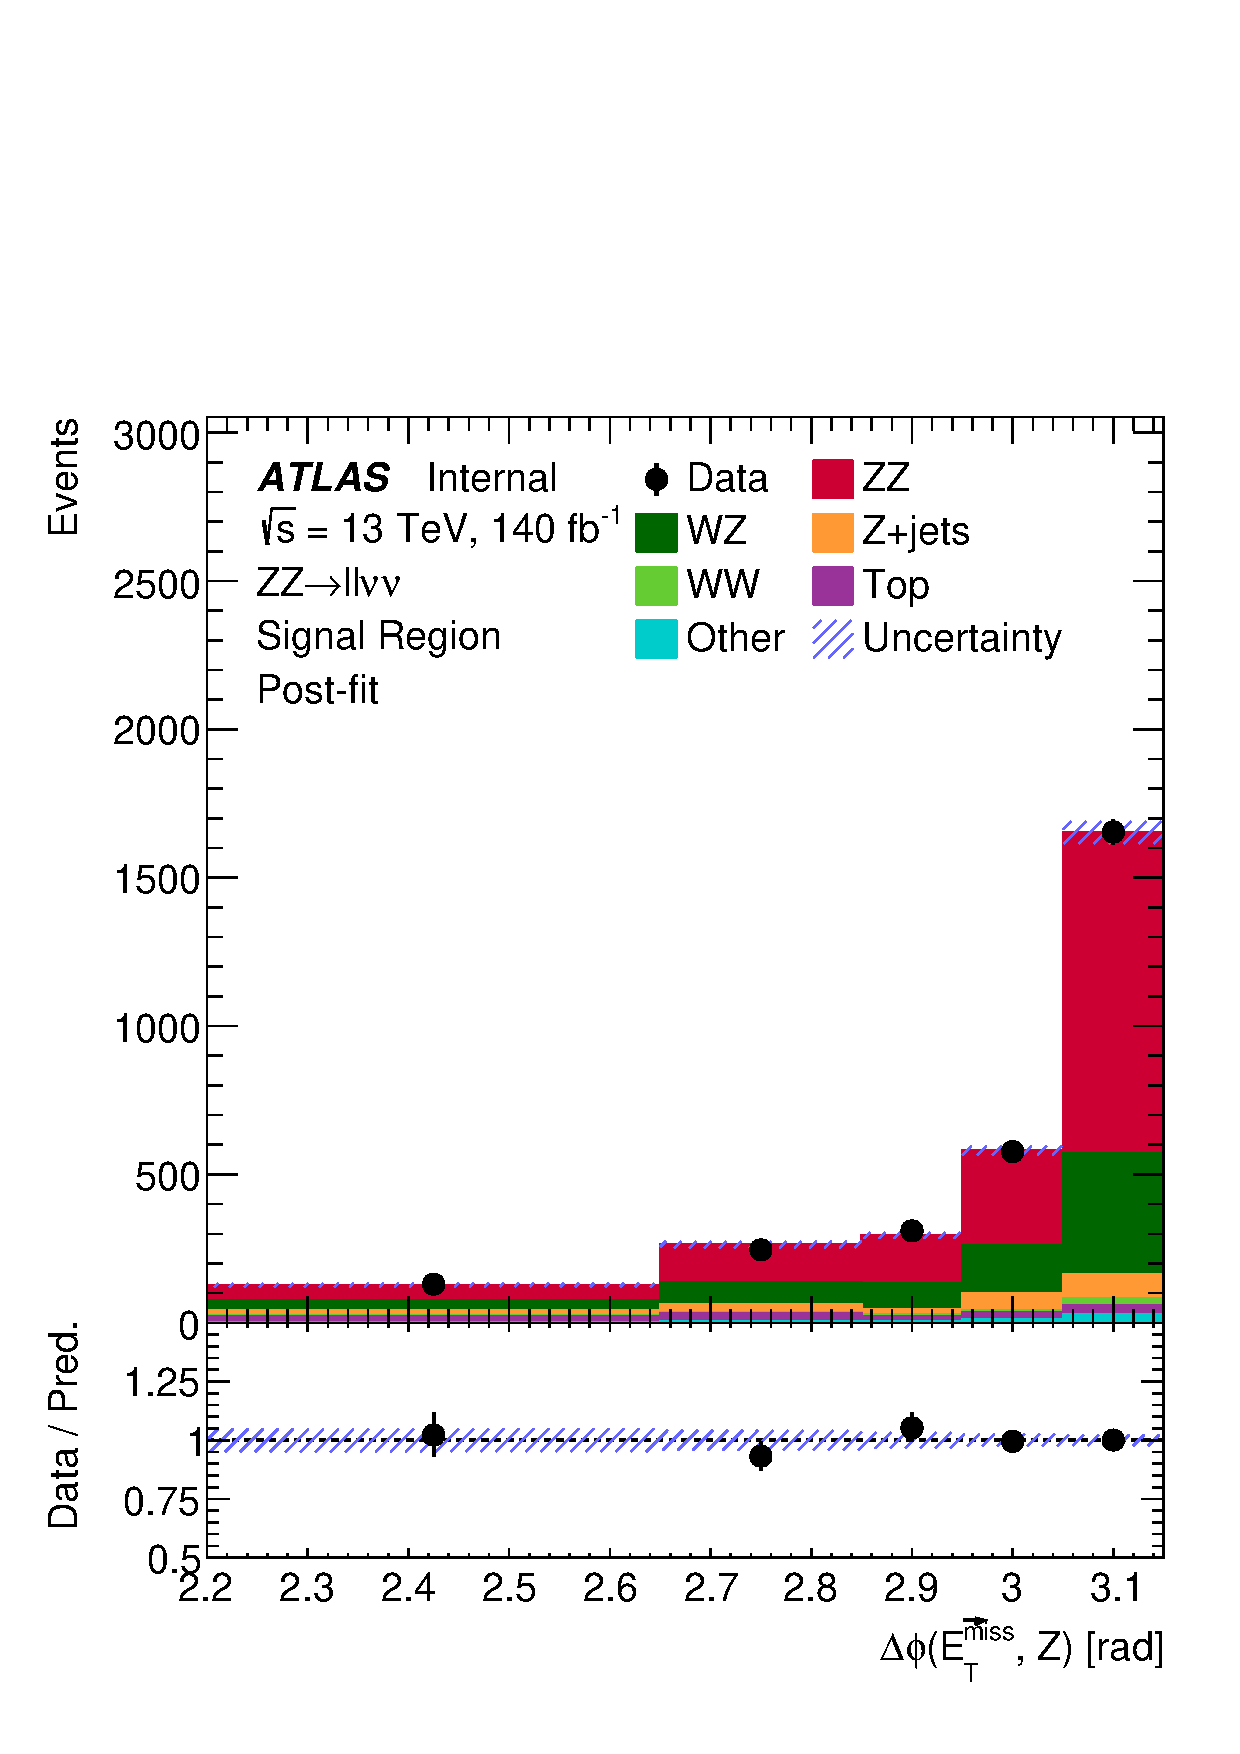
\includegraphics[width=0.32\linewidth]{figures/ch5-llvv/kin-distribution/SignalR_postFit-ZZ.pdf}
} 
    \subfloat[]{
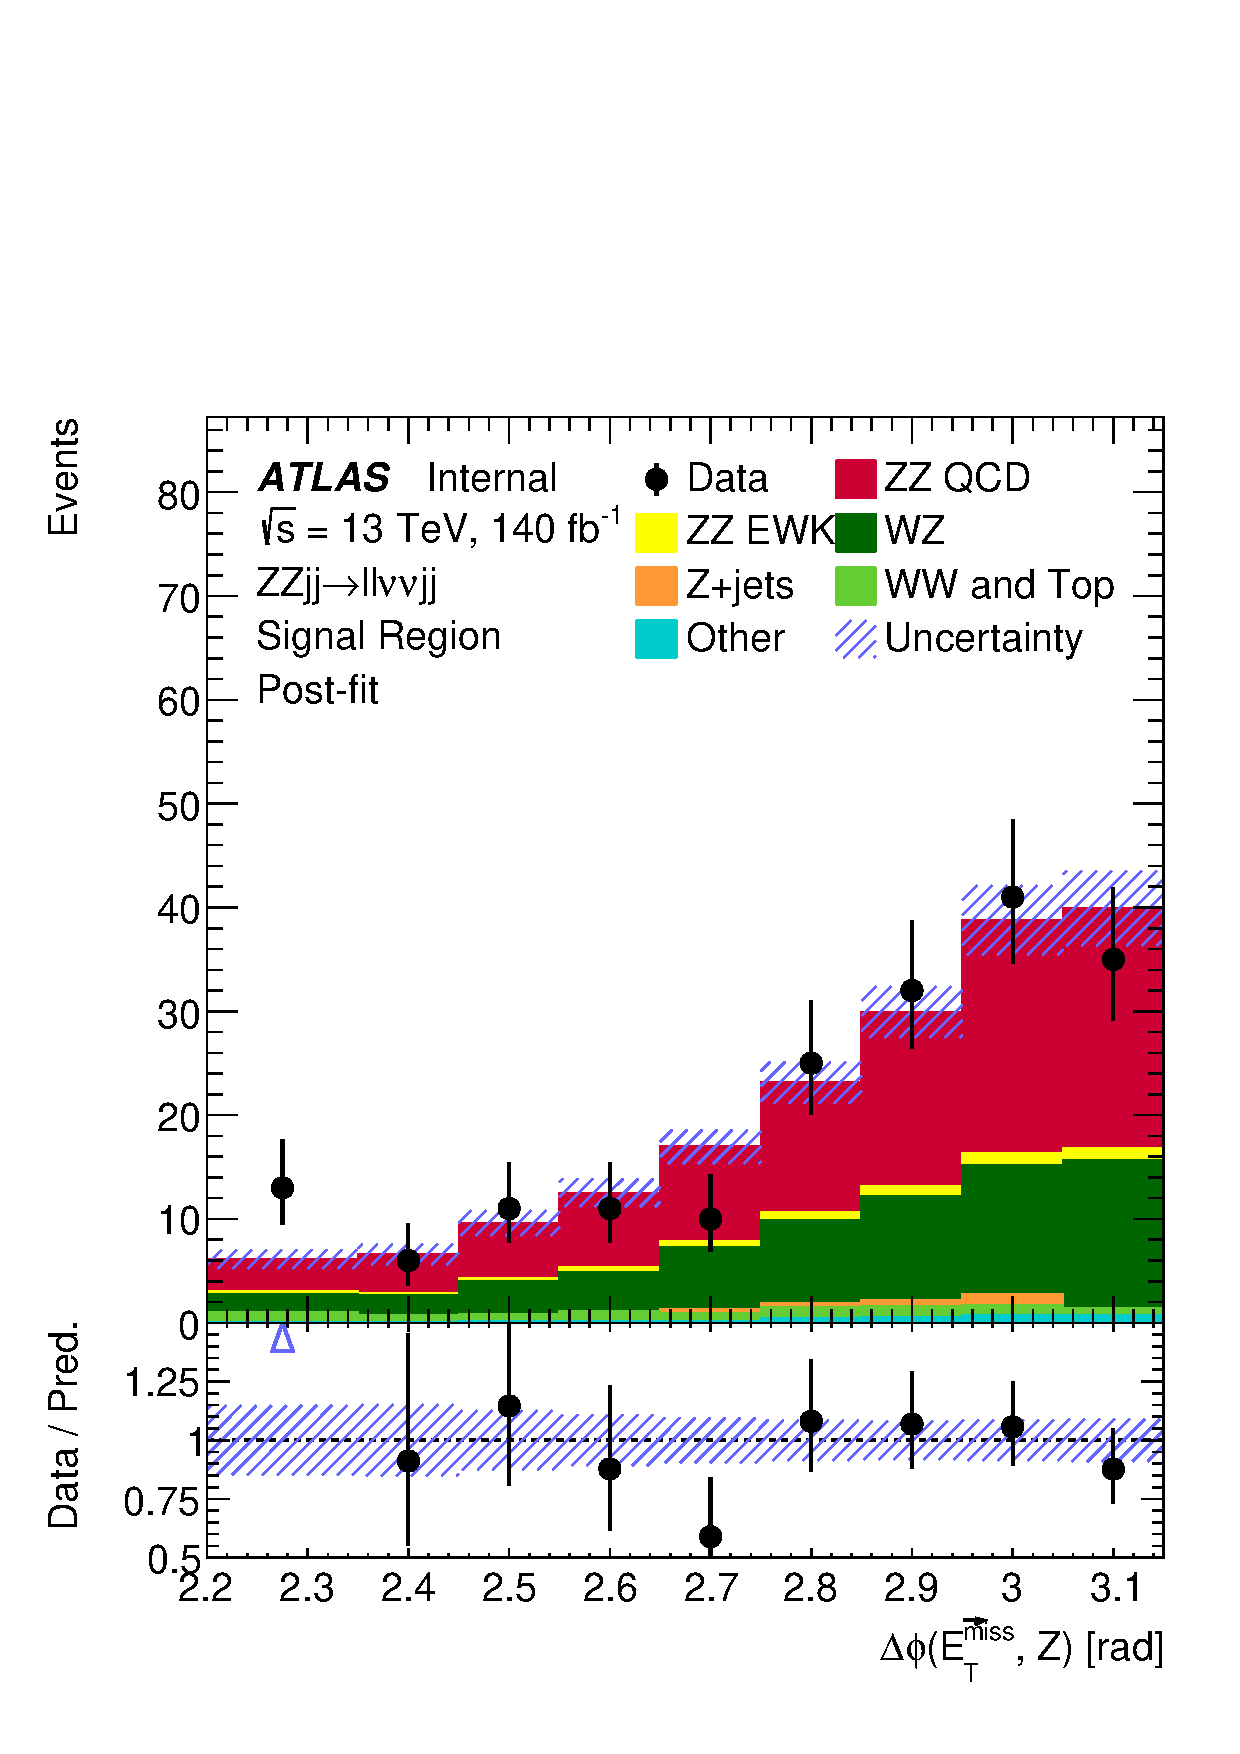
\includegraphics[width=0.32\linewidth]{figures/ch5-llvv/kin-distribution/SignalR_postFit-ZZjj.pdf}
}\\
    \subfloat[]{
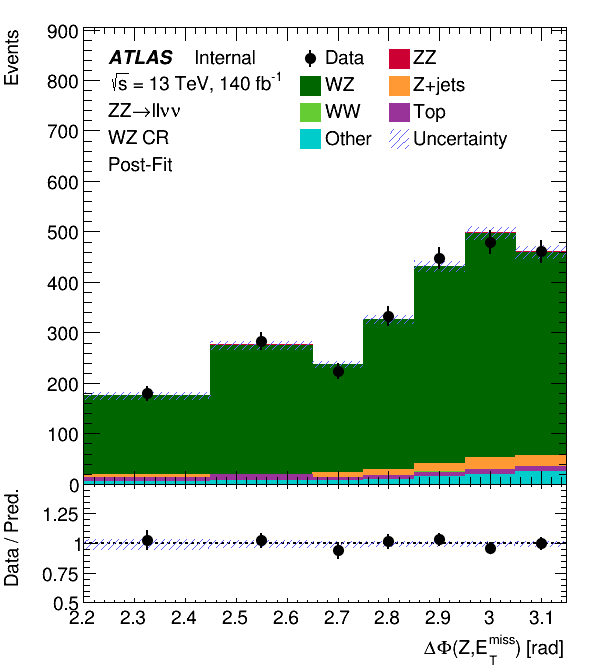
\includegraphics[width=0.325\linewidth]{figures/ch5-llvv/kin-distribution/WZ_postFit-ZZ.png}
}
    \subfloat[]{
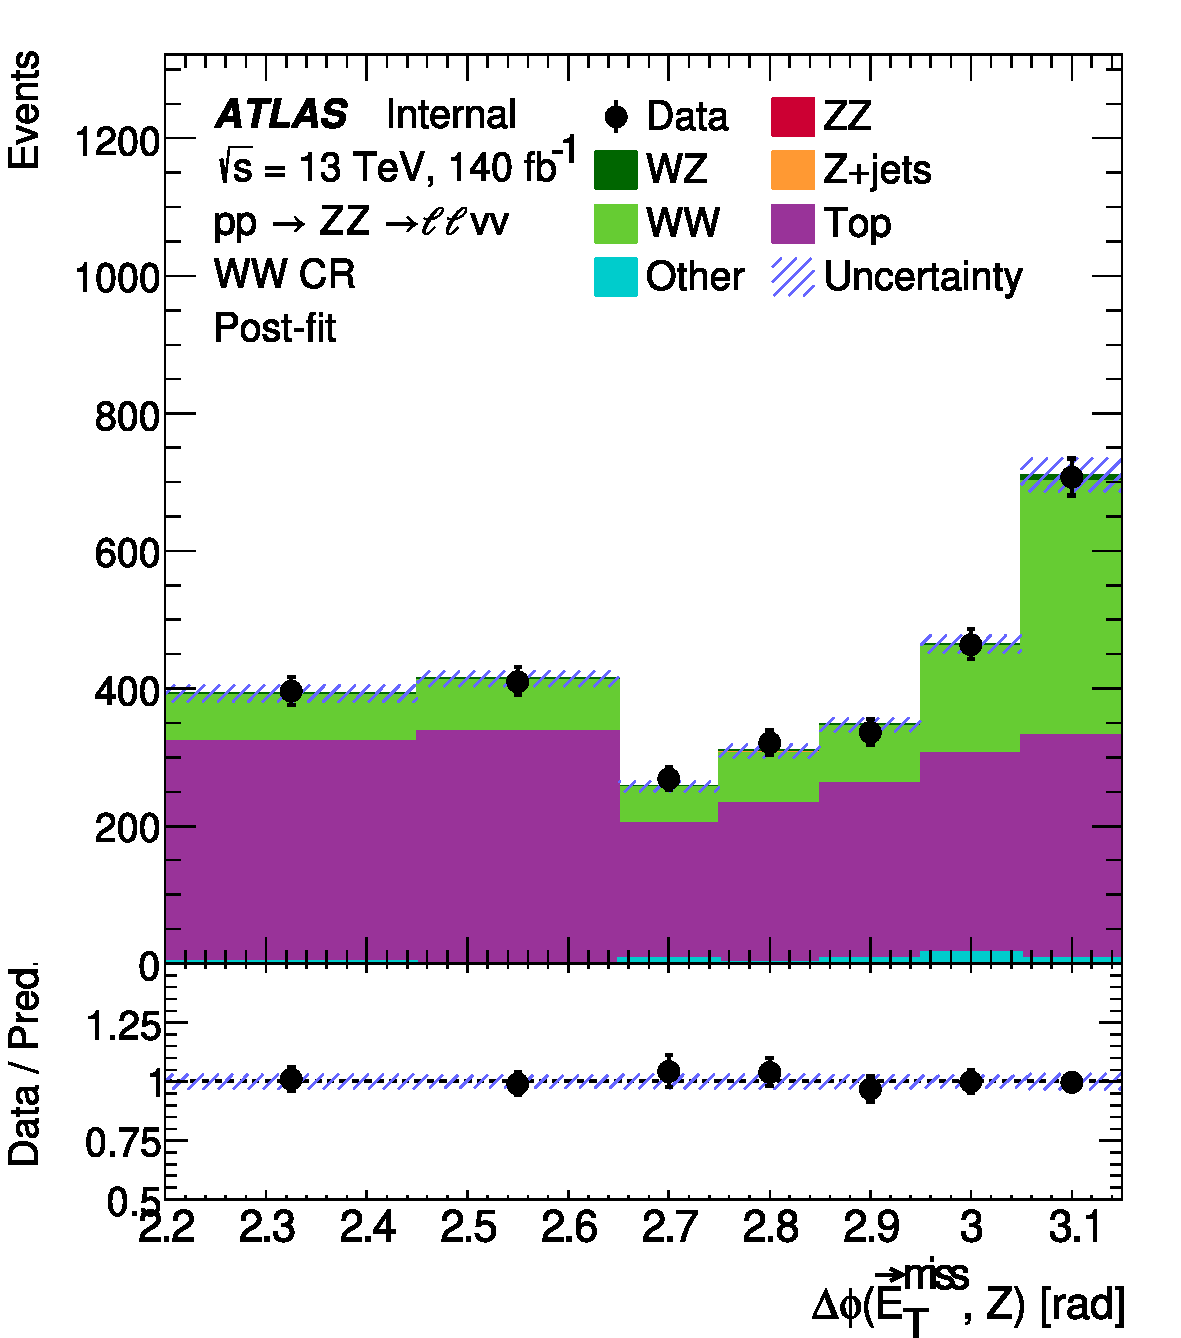
\includegraphics[width=0.32\linewidth]{figures/ch5-llvv/kin-distribution/EMU_A_postFit-ZZ.pdf}
}
    \subfloat[]{
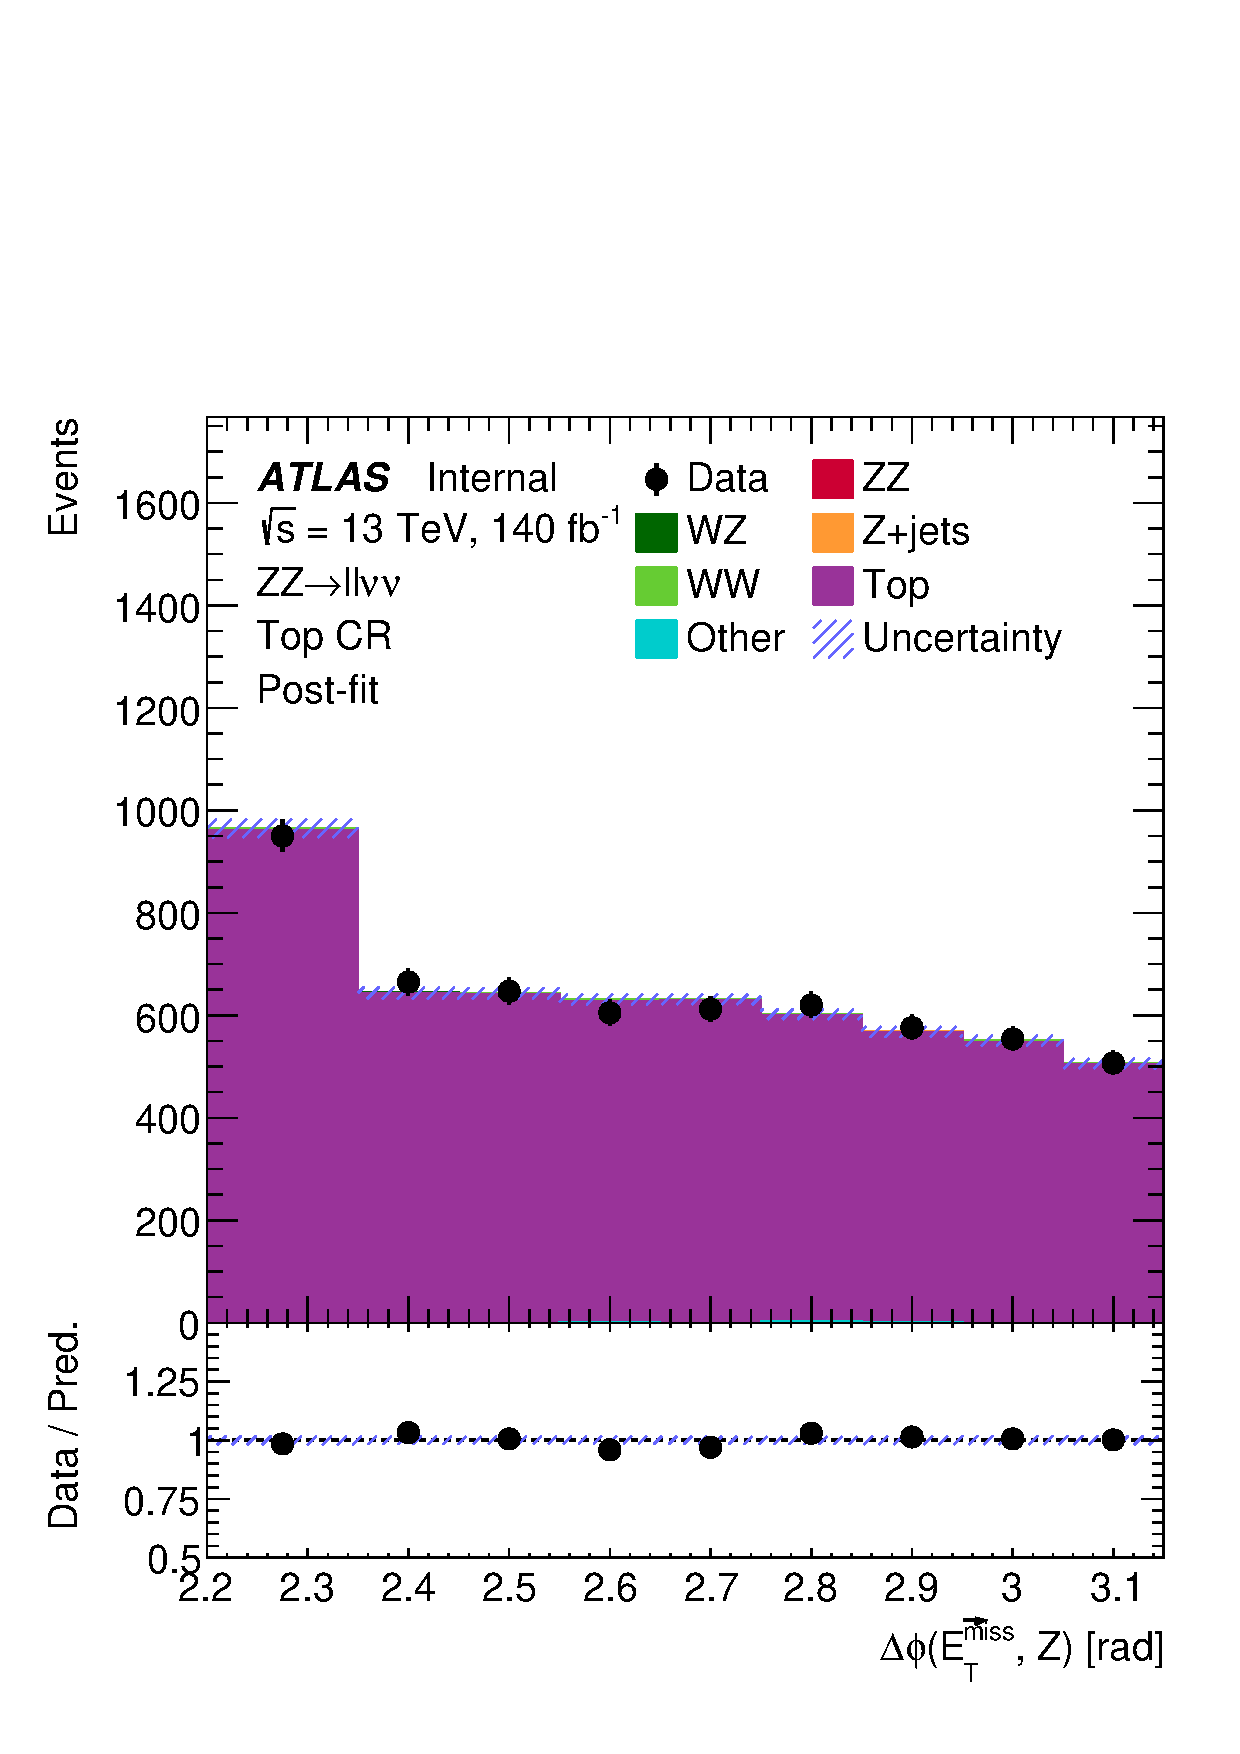
\includegraphics[width=0.32\linewidth]{figures/ch5-llvv/kin-distribution/EMU_B_postFit-ZZ.pdf}
}\\
    \subfloat[]{
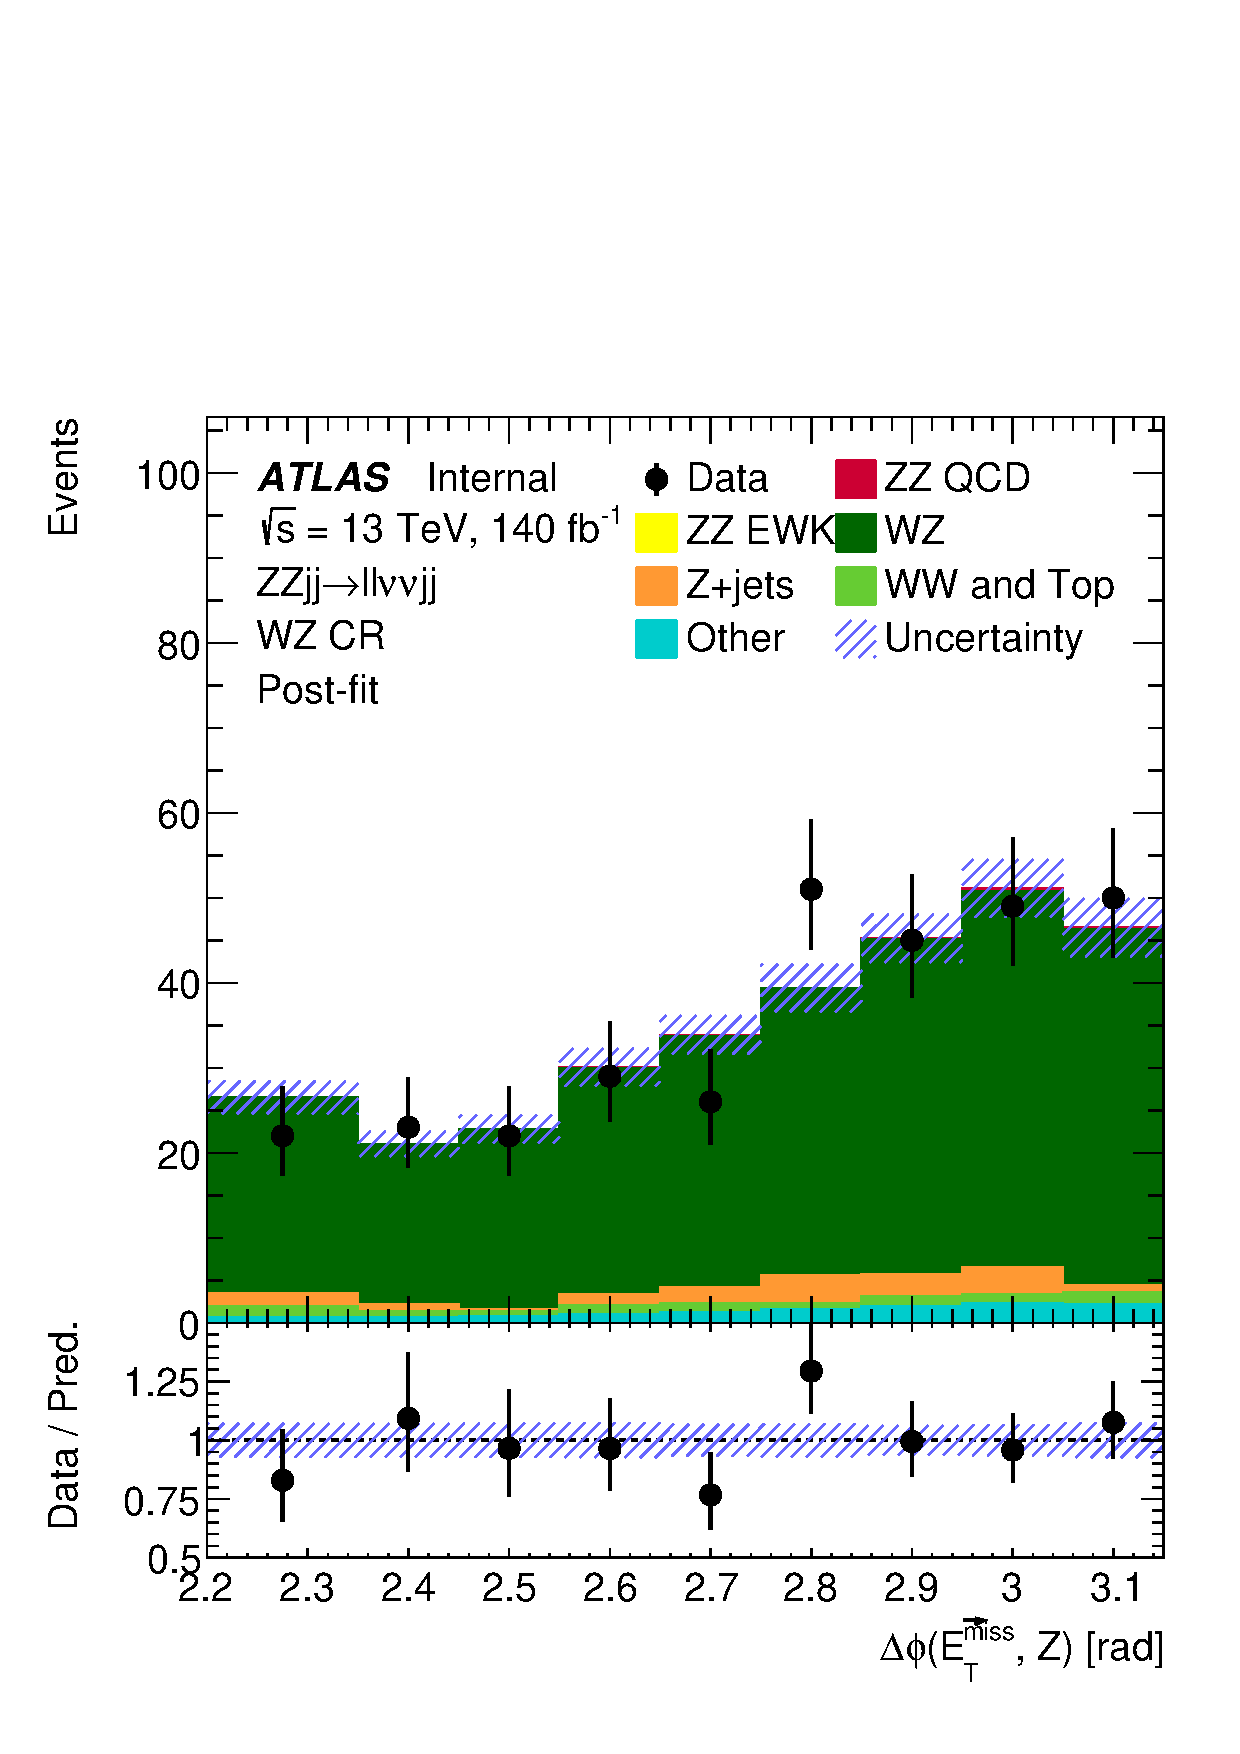
\includegraphics[width=0.325\linewidth]{figures/ch5-llvv/kin-distribution/WZ_postFit-ZZjj.pdf}
}
    \subfloat[]{
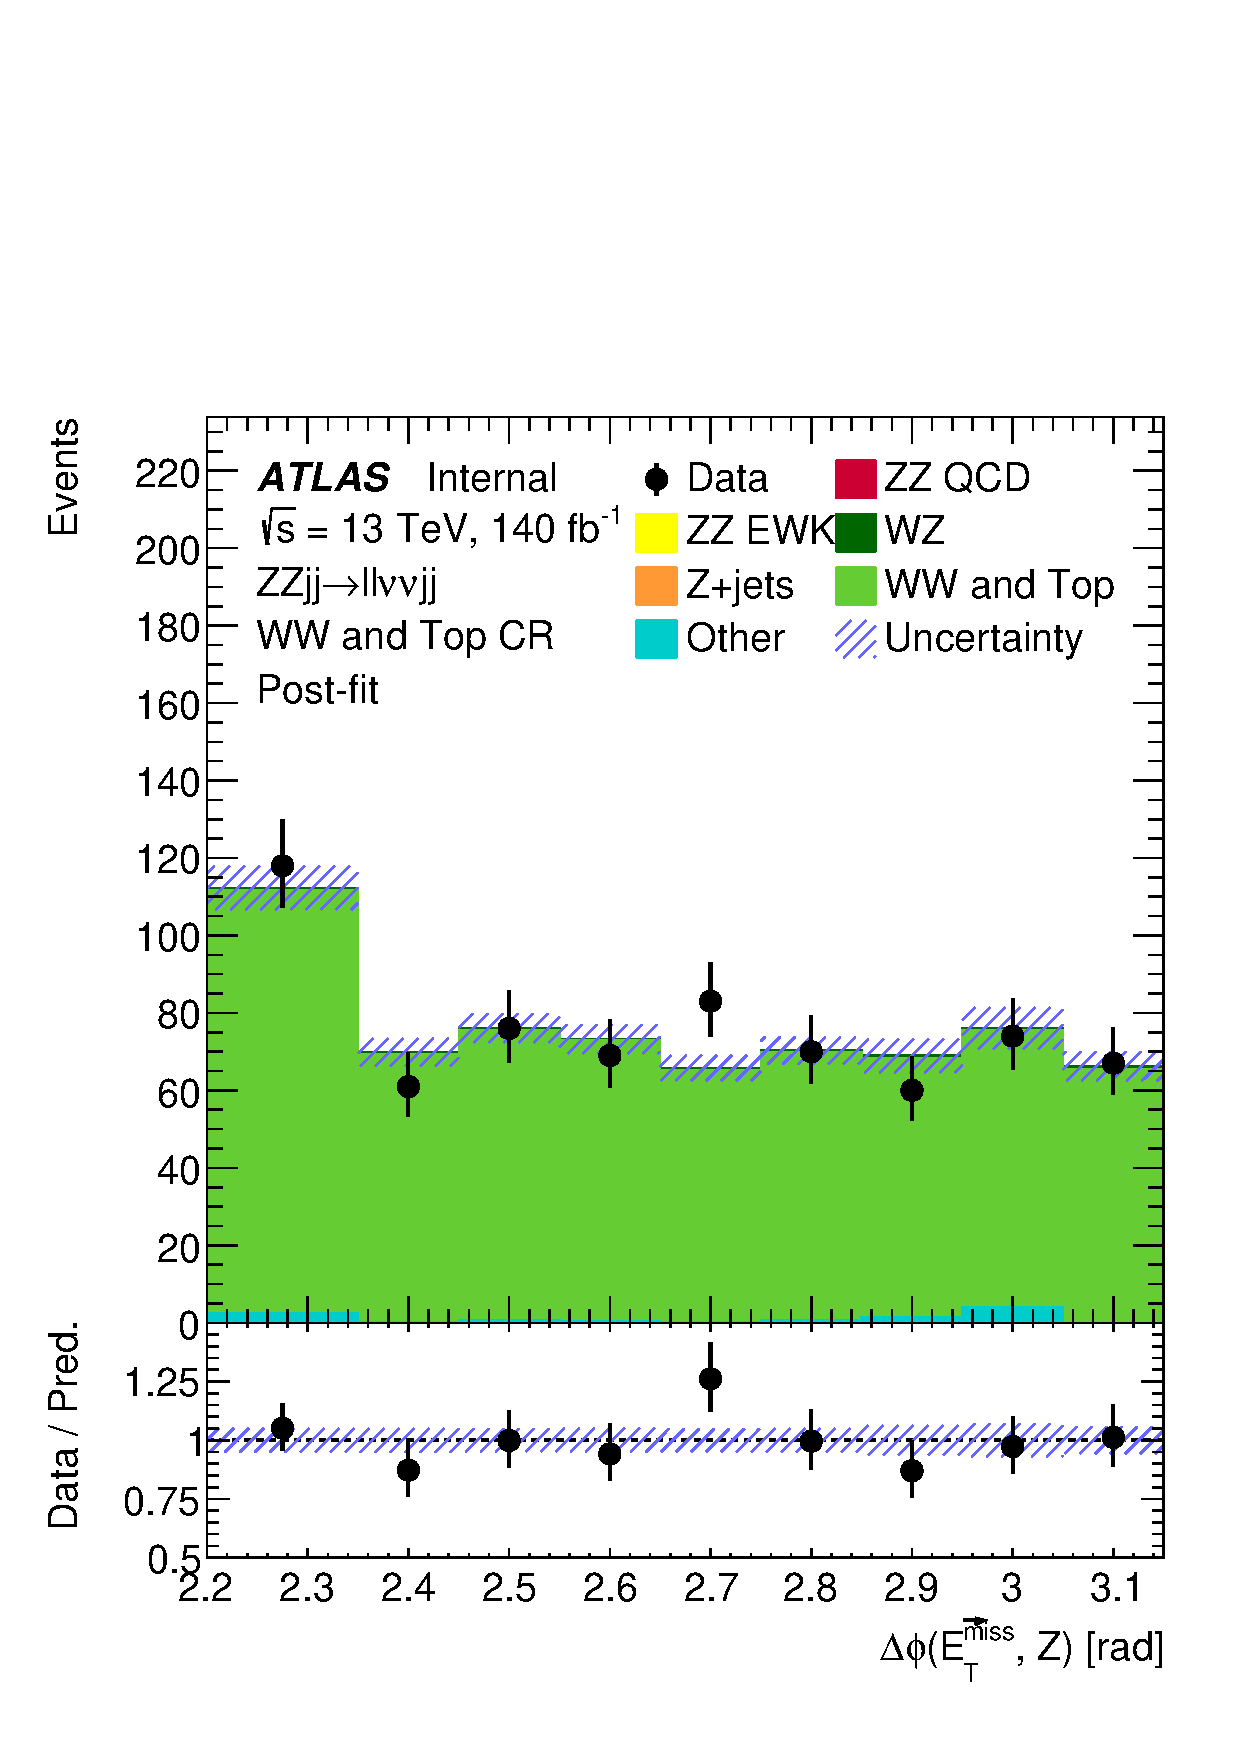
\includegraphics[width=0.325\linewidth]{figures/ch5-llvv/kin-distribution/EMU_postFit-ZZjj.pdf}
}
    \subfloat[]{
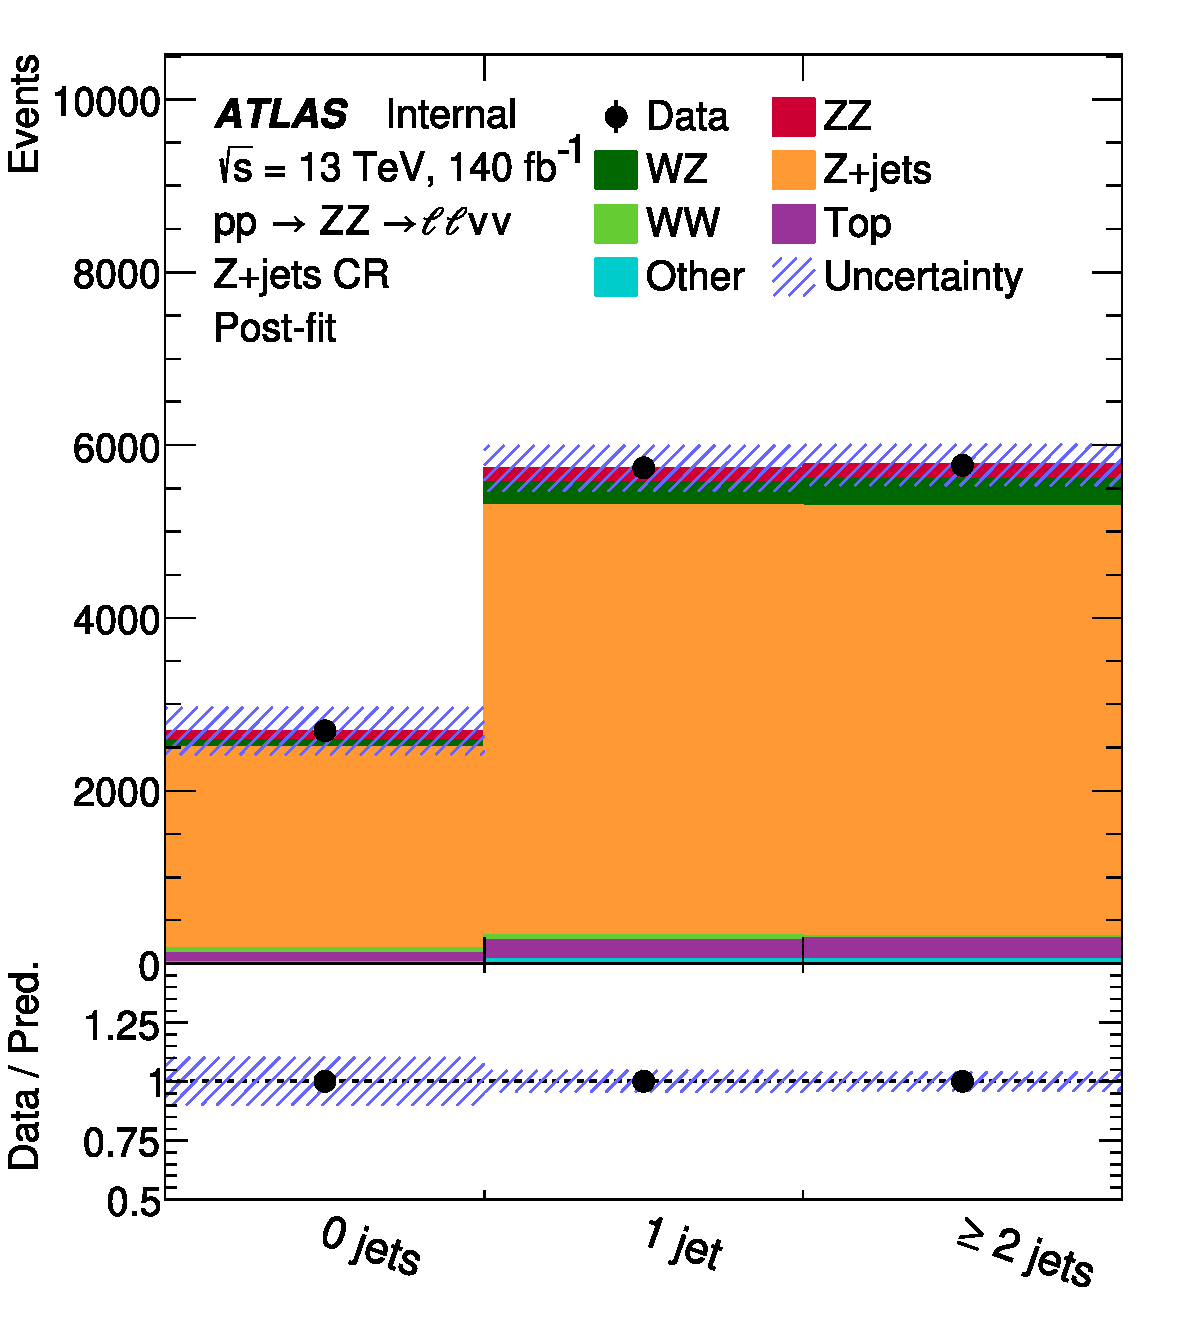
\includegraphics[width=0.325\linewidth]{figures/ch5-llvv/kin-distribution/Zj_VR_nJ_postFit-ZZ.pdf}
}
  \caption{The post-fit distributions of $\Delta\phi(\vec{E}_{\text{T}}^{\text{miss}}, \text{Z})$. Panels (a) and (b) show the signal regions for the inclusive $\text{ZZ}$ and $\text{ZZ}jj$ production, respectively. The ``Other'' category counts events from processes of $\text{ZZ} \to 4\ell, 2\ell 2q$, $\text{VVV}~(\text{V}=\text{W,Z})$, $\text{W}j$, $\text{Z} \to \tau\tau$, and $\text{WH}$. Figures (c), (d), and (e) illustrate the background CRs for inclusive $\text{ZZ}$ production, while panels (f) and (g) display the $\text{ZZ}jj$ CRs. Figure (h) presents the post-fit event yields for background events in the $\text{Z}$+0, 1, and $\ge 2$ jets CRs for the inclusive $\text{ZZ}$ analysis. Data points are shown with statistical error bars, while the shaded band represents the total post-fit uncertainty on the prediction, with combined statistical and systematic uncertainties.}
  \label{fig:postfit_observed_ZZCR}
\endminipage\hfill
\end{figure}

Additional post-fit kinematic distributions for the inclusive $\text{ZZ}$ SR are shown in the top row of Figure~\ref{fig:postfit_observed}: 
(a) the transverse momentum of the leading lepton, $p_{\text{T}}^{\text{leading-lepton}}$, 
(b) the missing transverse energy, $E_{\text{T}}^{\text{miss}}$, and 
(c) the azimuthal angle separation between the two charged leptons, $\Delta\phi(\ell, \ell)$. 
For the $\text{ZZ}jj$ SR, the bottom row shows: 
(d) the transverse momentum of the leading jet, $p_{\text{T}}^{\text{leading-jet}}$, 
(e) the invariant mass of the dijet system, $m_{jj}$, and 
(f) the transverse mass of the $\text{ZZ}$ system, $m_{\text{T}}^{\text{ZZ}}$. 

The data points are shown with statistical uncertainties, while the shaded band represents the total post-fit uncertainty in the prediction, including both statistical and systematic components. 
Overall, good agreement between data and MC predictions is observed across all distributions.


\begin{figure}[!htbp]
\minipage{1\textwidth}
\centering
   \subfloat[]{
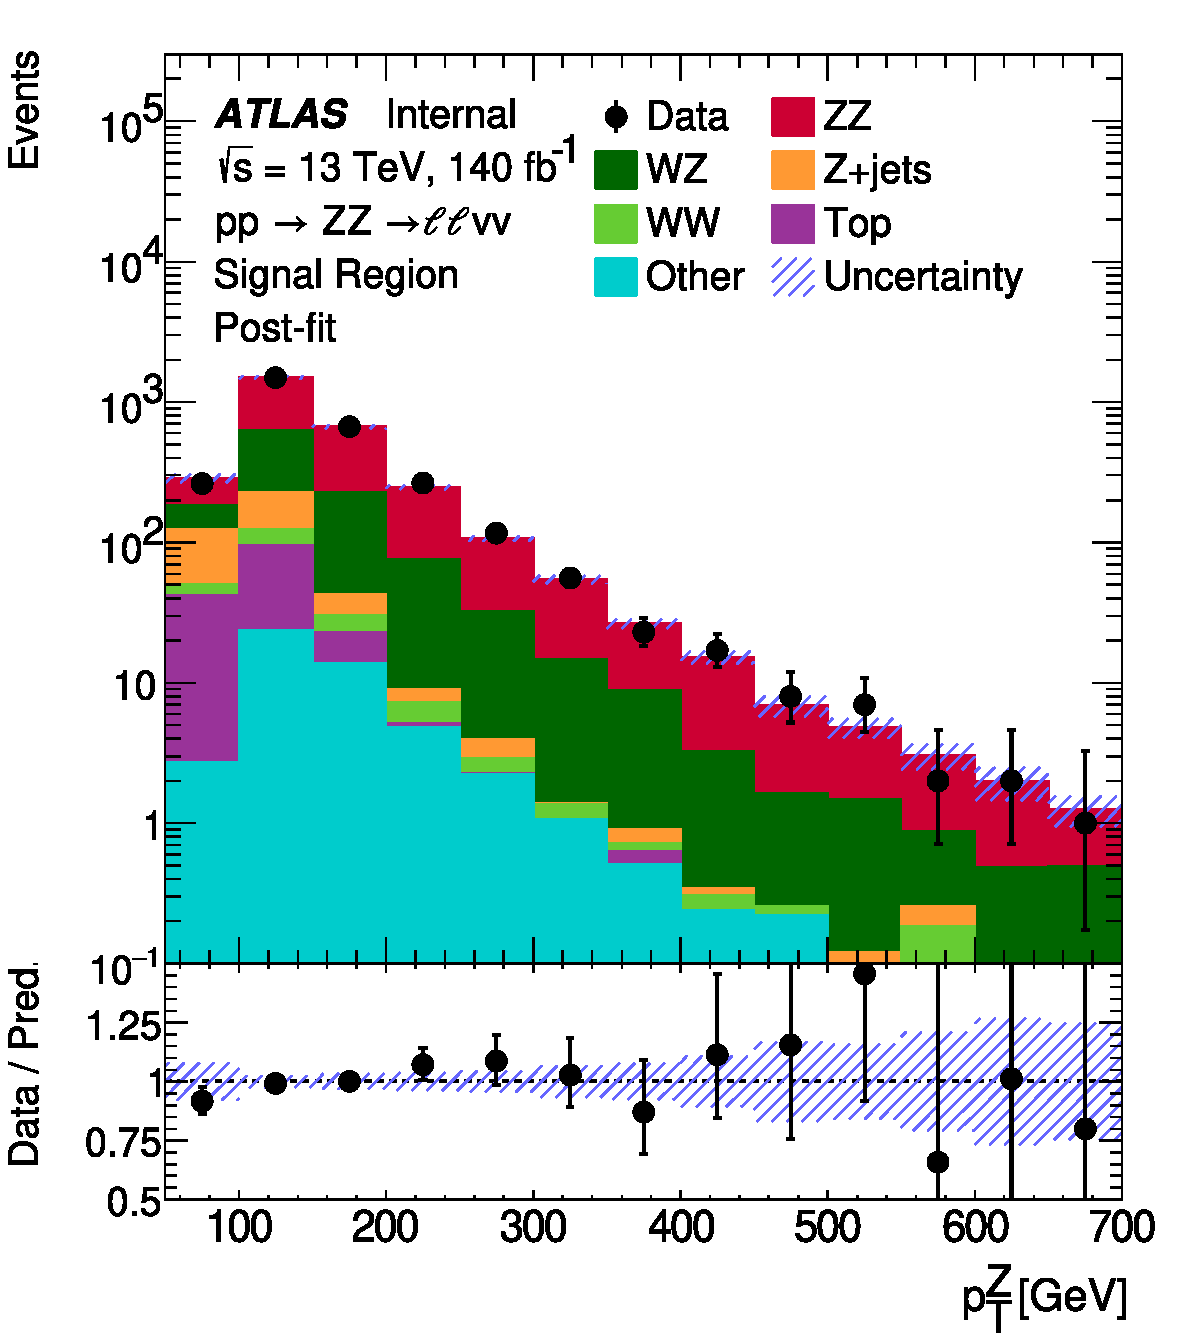
\includegraphics[width=0.32\linewidth]{figures/ch5-llvv/kin-distribution/Val_green_ptZ50_postFit-ZZ.pdf}
}
    \subfloat[]{
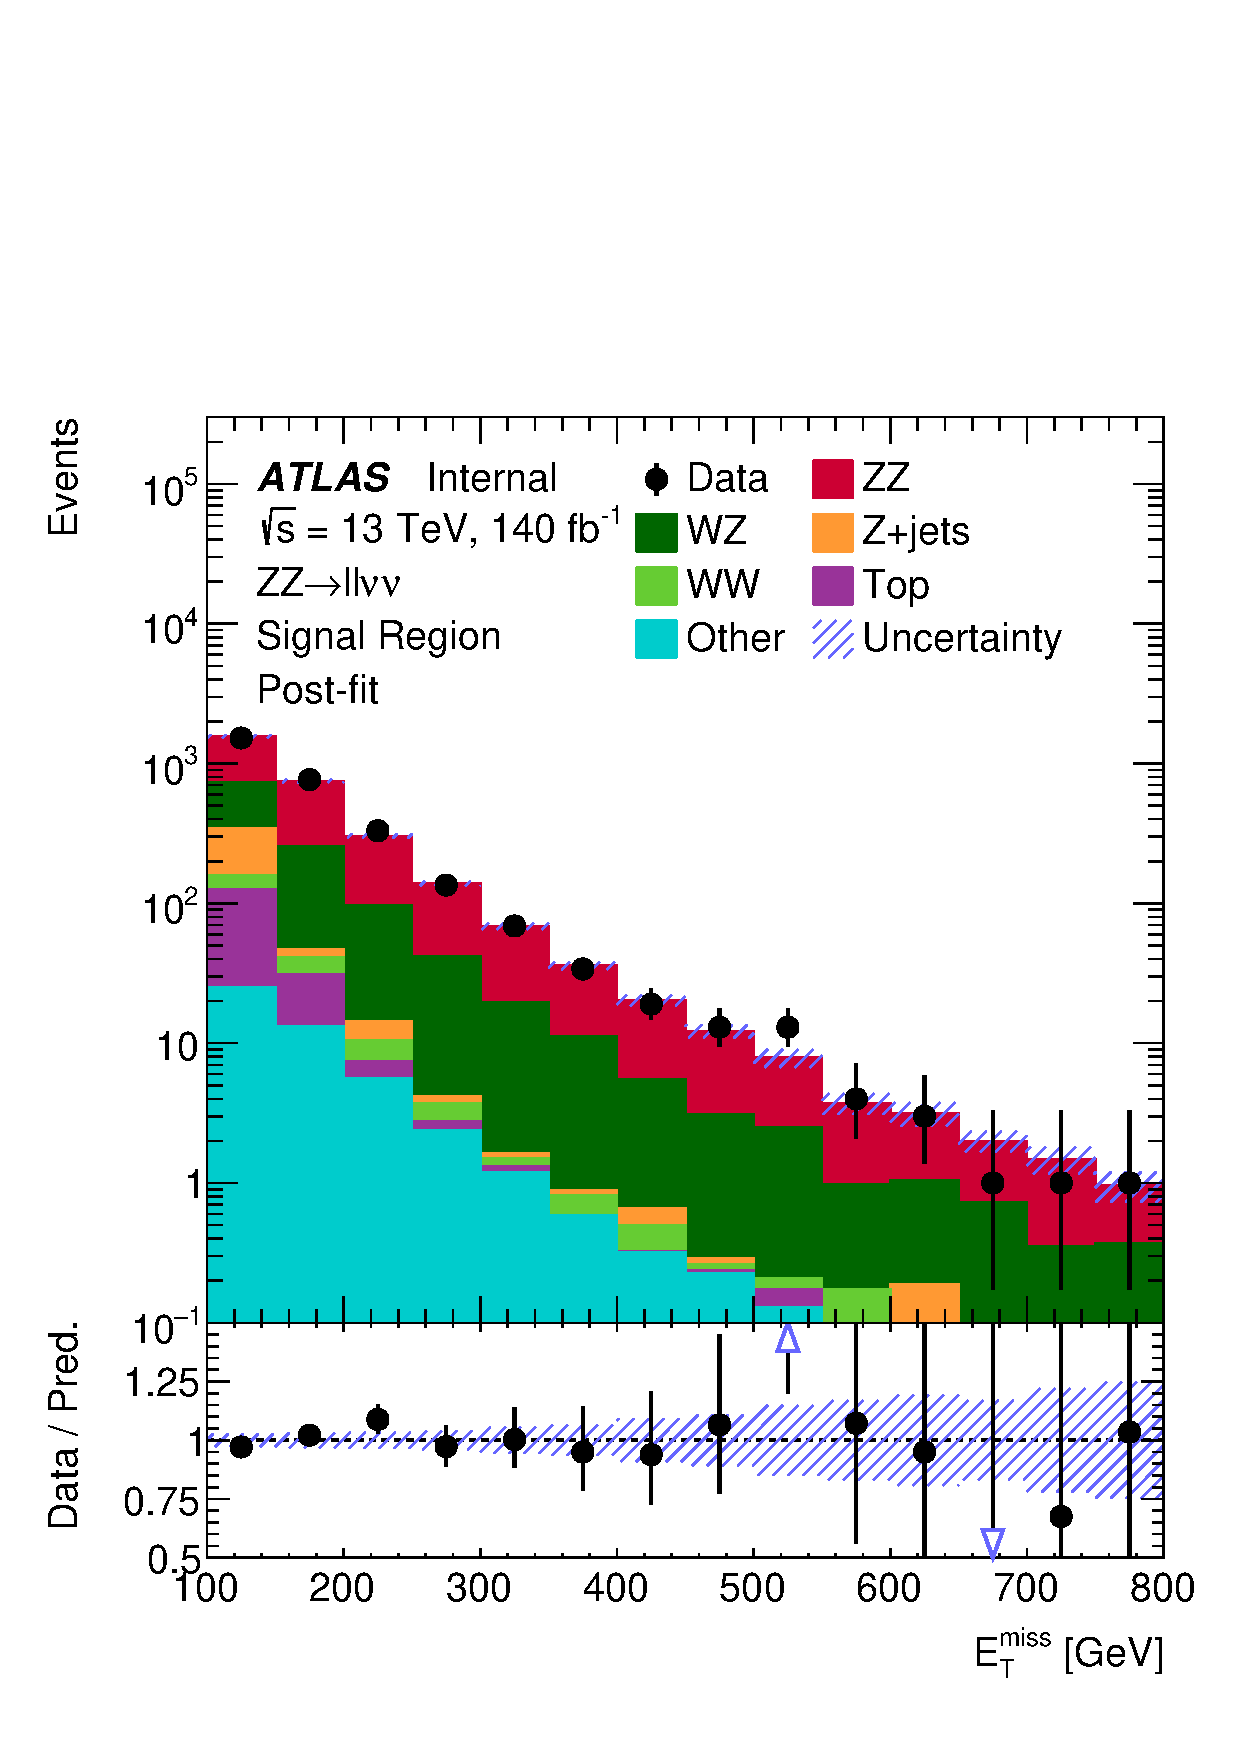
\includegraphics[width=0.32\linewidth]{figures/ch5-llvv/kin-distribution/Val_green_met50_postFit-ZZ.pdf}
}
    \subfloat[]{
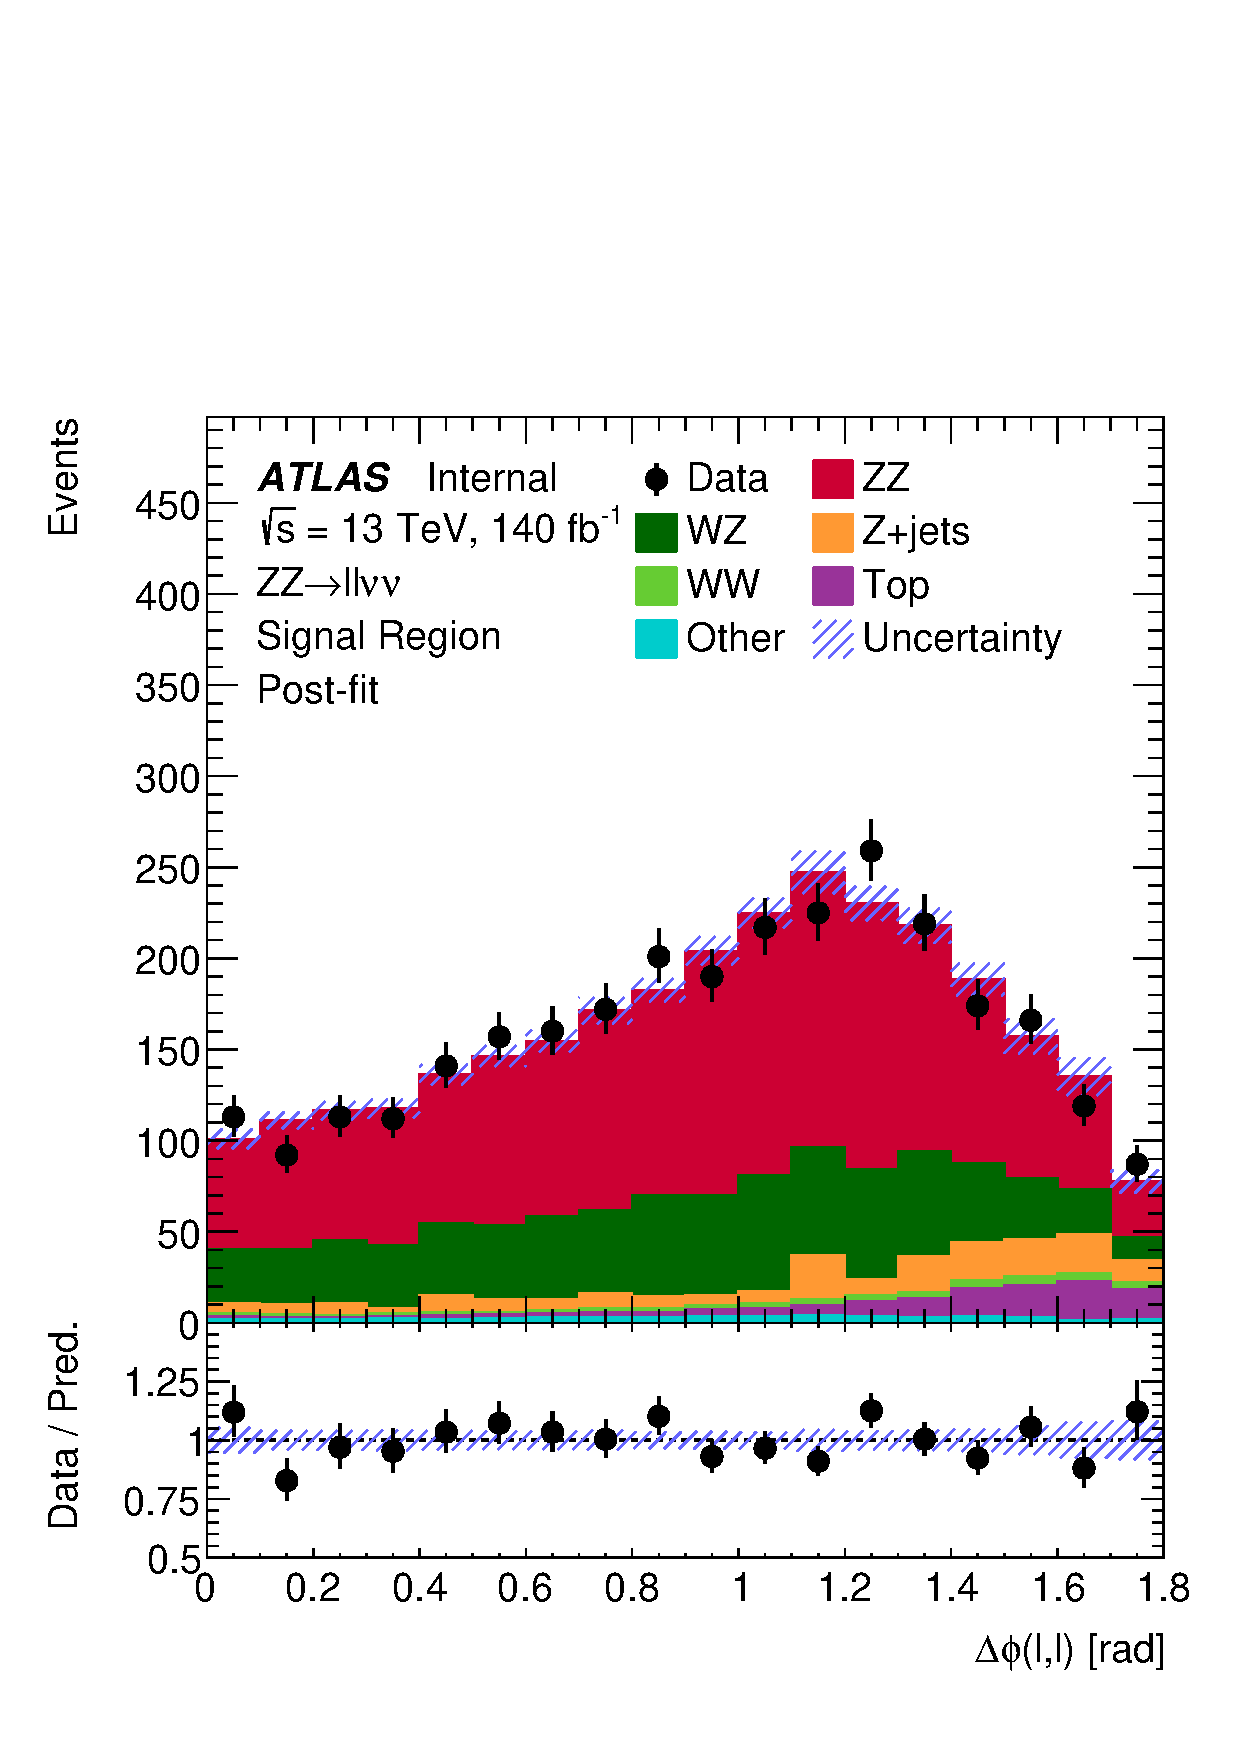
\includegraphics[width=0.32\linewidth]{figures/ch5-llvv/kin-distribution/Val_green_dPhill50_postFit-ZZ.pdf}
}\\
    \subfloat[]{
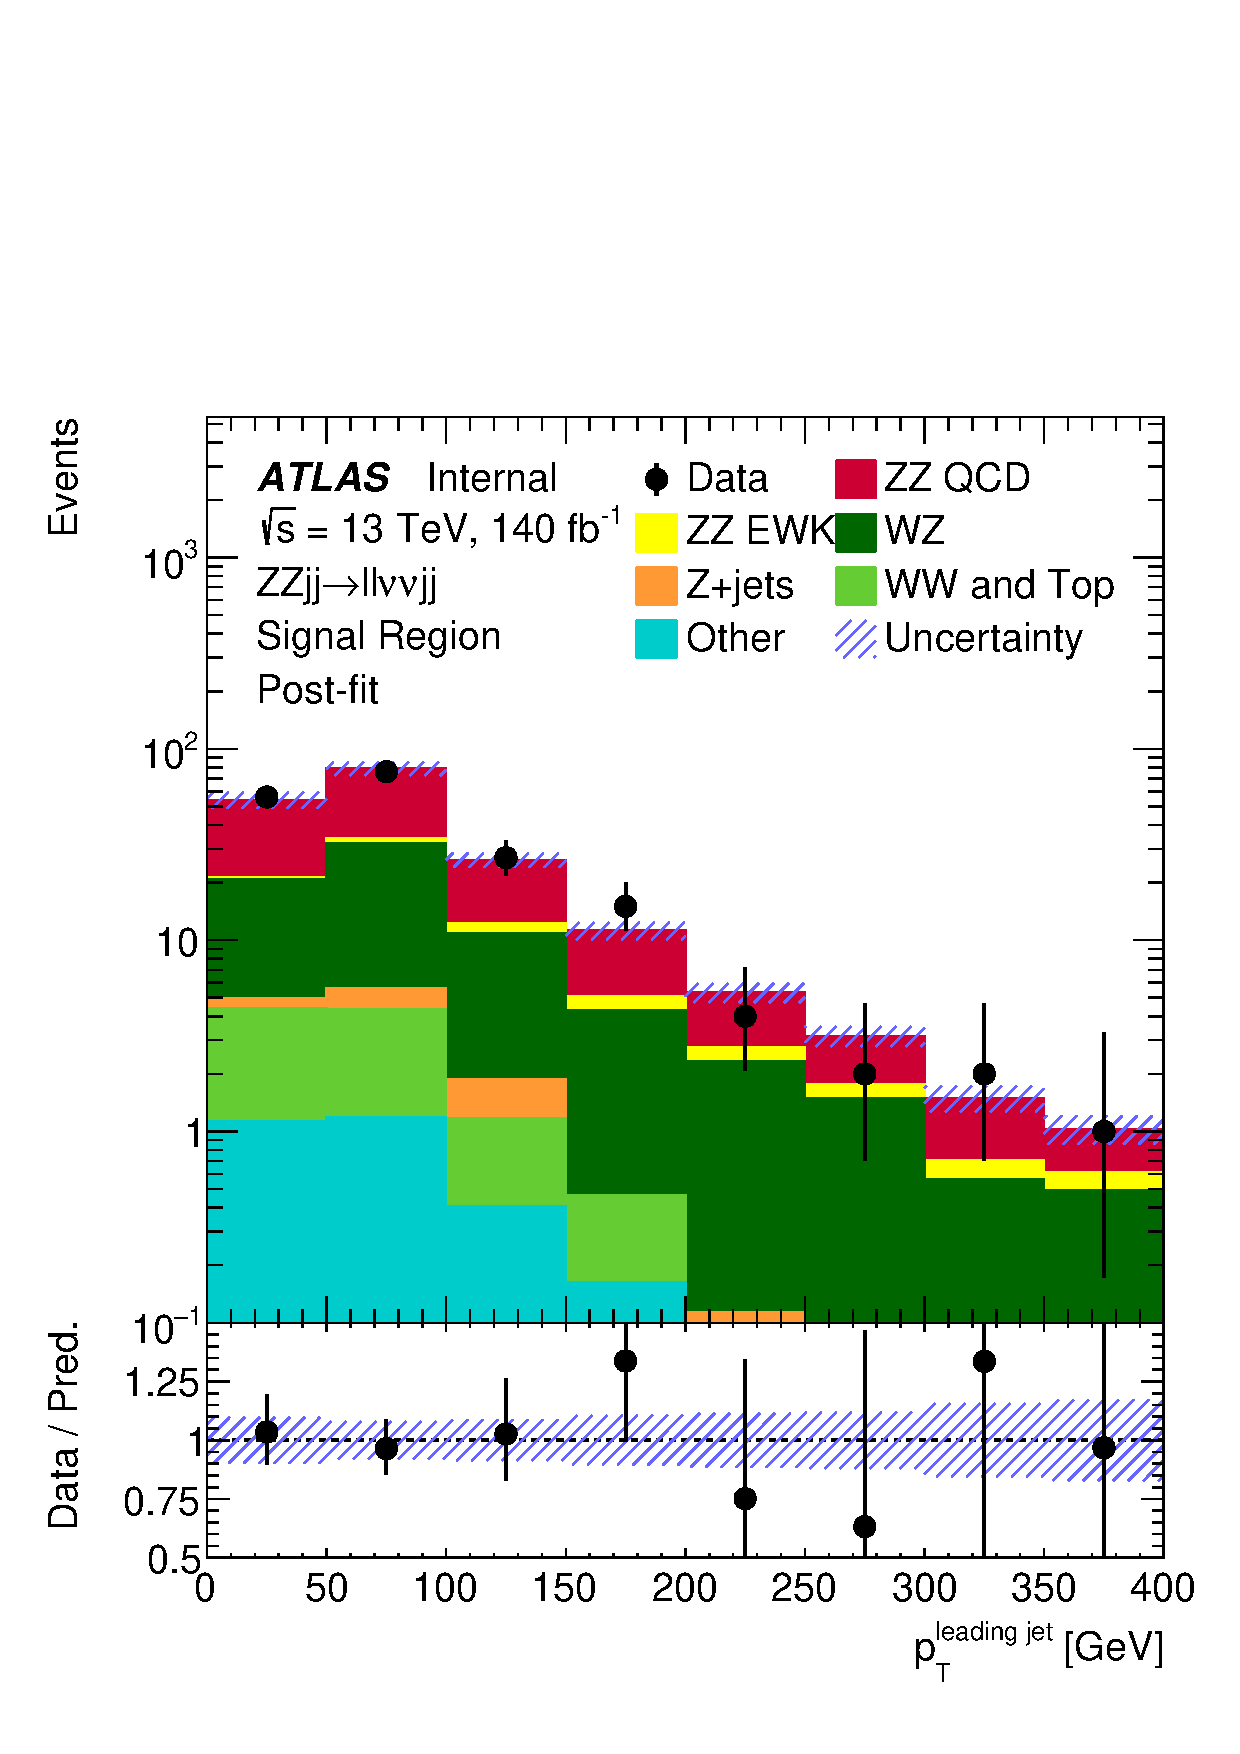
\includegraphics[width=0.32\linewidth]{figures/ch5-llvv/kin-distribution/SignalR_Jpt50_postFit-ZZjj.pdf}
}
    \subfloat[]{
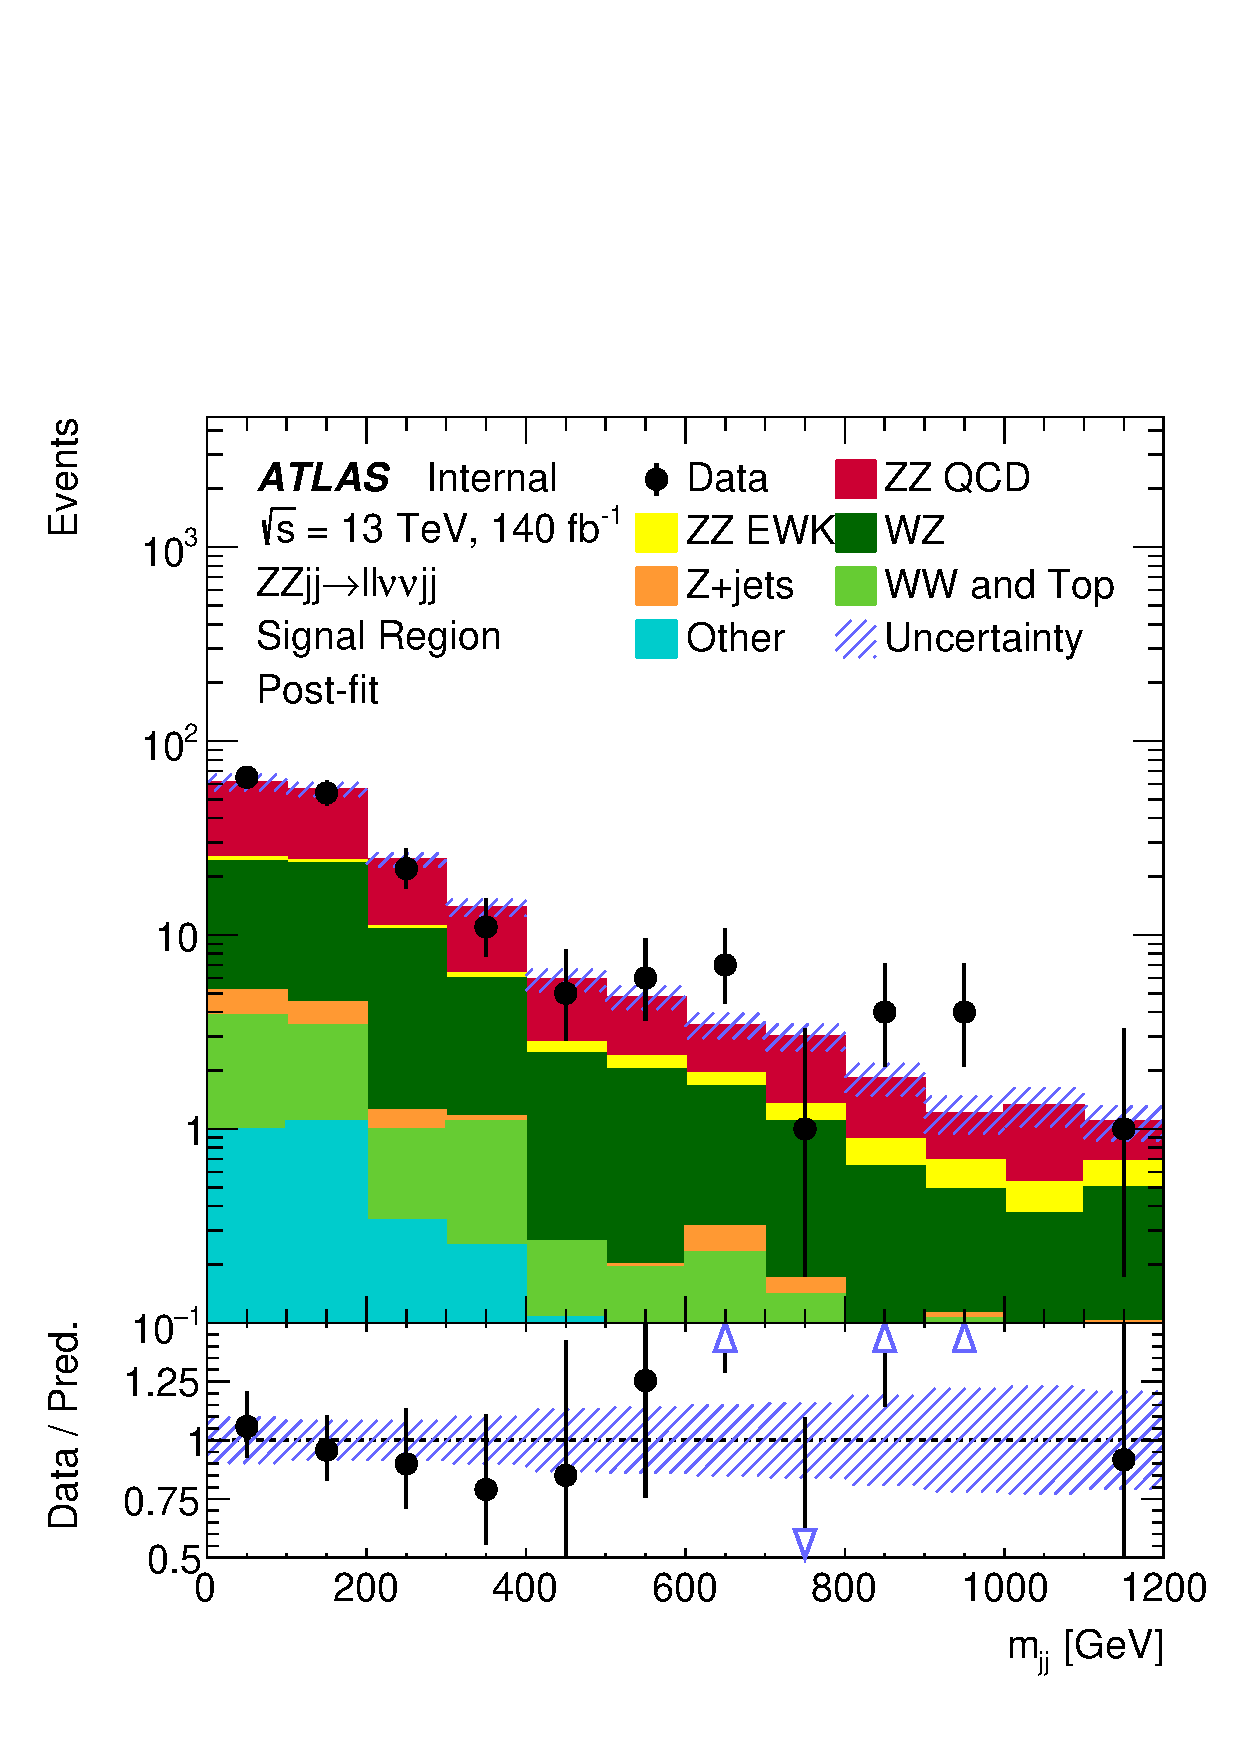
\includegraphics[width=0.32\linewidth]{figures/ch5-llvv/kin-distribution/SignalR_mjj100_postFit-ZZjj.pdf}
}
    \subfloat[]{
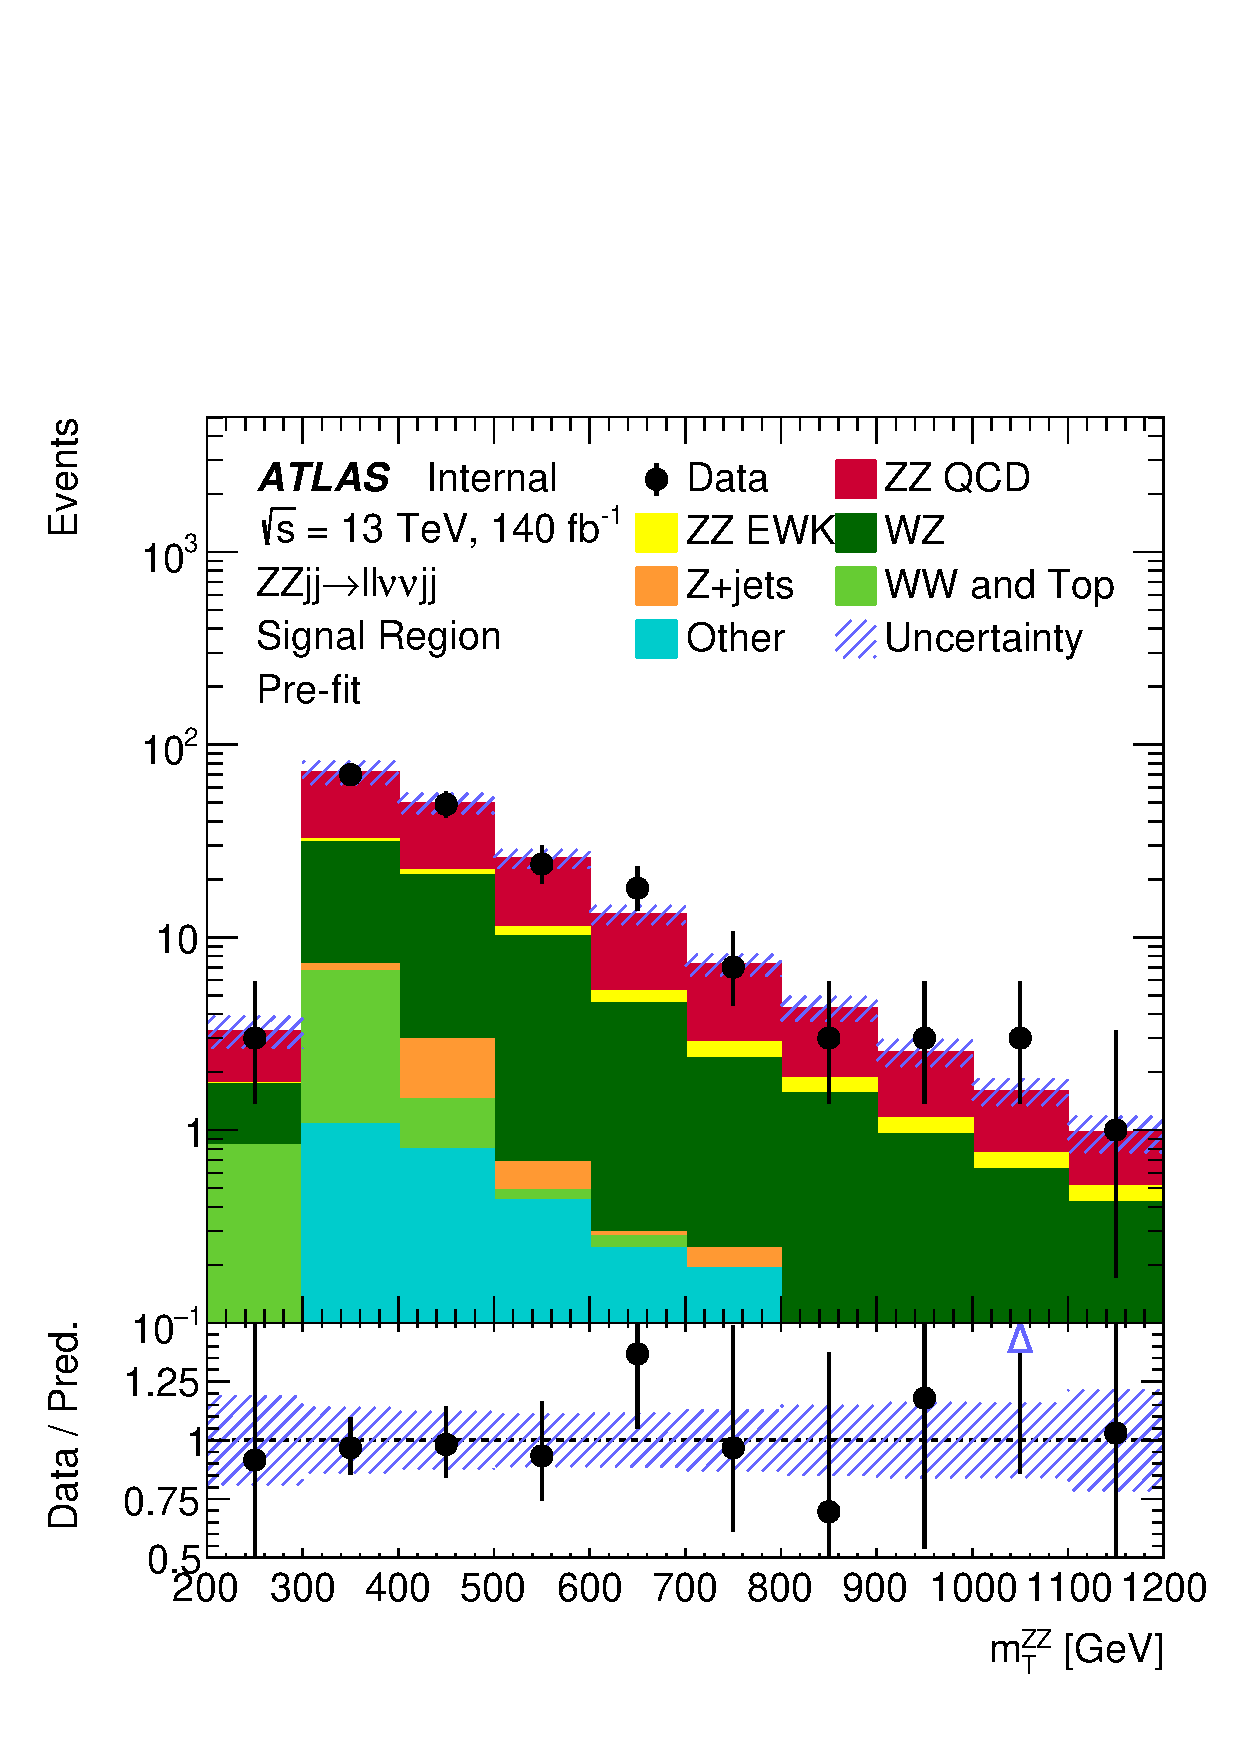
\includegraphics[width=0.32\linewidth]{figures/ch5-llvv/kin-distribution/SignalR_mtzz100_log-ZZjj.pdf}
}
  %\caption{Post-fit kinematic distributions for the inclusive $ZZ$ SR are shown in the top row: (a) the transverse momentum of the leading lepton $p_\text{T}^\text{leading-lepton}$, (b) the missing transverse energy $E_\text{T}^\text{miss}$ and (c) the azimuthal angle separation between two charged leptons $\Delta\phi(\ell, \ell)$. For the $ZZjj$ SR, the bottom row shows: (d) the leading jet $p_\text{T}^\text{leading-jet}$, (e) the invariant mass of the dijet system $m_\text{jj}$, 
  \caption{Post-fit kinematic distributions for the inclusive $\text{ZZ}$ SR are shown in the top row: (a) the transverse momentum of the lepton pair, (b) the missing transverse energy $E_{\text{T}}^{\text{miss}}$, and (c) the azimuthal angle separation between two charged leptons $\Delta\phi(\ell, \ell)$. For the $\text{ZZ}jj$ SR, the bottom row shows: (d) the leading jet $p_{\text{T}}^{\text{leading-jet}}$, (e) the invariant mass of the dijet system $m_{jj}$, 
  and (f) the transverse mass of the $\text{ZZ}$ system $m_{\text{T}}^{\text{ZZ}}$. The data points are shown with statistical error bars, while the shaded band represents the total post-fit uncertainty in the prediction, with combined statistical and systematic uncertainties.}
  \label{fig:postfit_observed}
\endminipage\hfill
\end{figure}


The fiducial cross-sections for the processes $\text{ZZ} \to \ell\ell\nu\nu$ and $\text{ZZ}jj \to \ell\ell\nu\nu jj$ in their respective fiducial phase spaces are calculated by multiplying the measured signal strengths ($\mu_{\text{S}}^{\text{ZZ}}$ and $\mu_{\text{S}}^{\text{ZZ}jj}$) by the SM cross-section predictions as shown in Table~\ref{tab:sherpa-xs}.

The measured fiducial cross-section for the inclusive $\text{ZZ} \to \ell\ell\nu\nu$ production process is found to be
\begin{equation*}
\sigma_{\text{ZZ}}^{\text{fid}} = 21.03 \pm 0.73_{\text{stat}} \pm 0.57_{\text{exp}} \pm 0.18_{\text{theory}} \pm 0.18_{\text{lumi}}~\text{fb},
\end{equation*} 
where the uncertainty is separated into the data statistical uncertainty (stat), the uncertainty from experimental systematic uncertainties (exp), the uncertainty from theory systematic uncertainties (theory), and the luminosity uncertainty (lumi). 
The measured cross-section is in agreement with the SM prediction of $20.1 \pm 1.1~\text{fb}$ from \textsc{Sherpa}+\textsc{MadGraph5} and $21.03 \pm 0.30~\text{fb}$ from \textsc{Matrix}. 

For the $\text{ZZ}jj \to \ell\ell\nu\nu jj$ production process, the measured fiducial cross-section is 
\begin{equation*}
\sigma_{\text{ZZ}jj}^{\text{fid}} = 0.96^{+0.15}_{-0.11\text{ (stat)}} \pm 0.10_{\text{exp}} \pm 0.04_{\text{theory}} \pm 0.01_{\text{lumi}}~\text{fb}.
\end{equation*}
This is compatible with the theoretical prediction of $0.94 \pm 0.20~\text{fb}$ from \textsc{Sherpa}+\textsc{MadGraph5}. 

The $\text{ZZ} \to \ell\ell\nu\nu$ fiducial production cross-section is extrapolated to the total phase space, using the fiducial acceptance reported in Table~\ref{tab:zz-xs} and the branching ratio~\cite{Zyla:2020zbs} of the $\text{ZZ}$ decay mode $\text{ZZ} \to 2\ell 2\nu$. 

The total $pp \to \text{ZZ}$ production is found to be:
\begin{equation*}
\sigma^{\text{total}}_{\text{measured}}(pp \to \text{ZZ}) = 15.38 \pm 0.81~\text{pb}.
\end{equation*}
This measurement is in agreement with the SM prediction calculated using \textsc{Matrix}: $\sigma^{\text{total}}_{\text{SM}}(pp \to \text{ZZ}) = 15.40 \pm 0.38~\text{pb}$.


